\begin{figure*}[t]
\centering
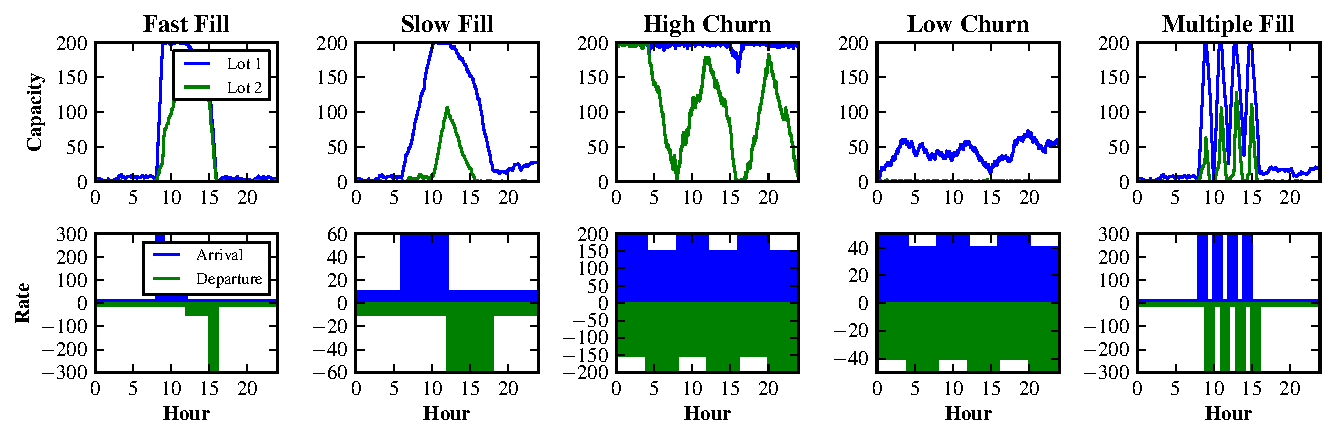
\includegraphics[width=\textwidth]{./simulator/figures/lots.pdf}

\caption{\textbf{Description of each type of lot simulated.} Five different
lots with different behaviors were used during simulations.}

\label{fig-lotsdescription}
\end{figure*}

\section{Evaluation}
\label{sec-evaluation}

We evaluate PocketParker in three ways. First, we conducted a controlled
experiment to determine the best parameter settings for our event detector.
Second, we implemented a parking lot simulator to experiment with various
kinds of lots and vary the monitored fraction and other parameters. Finally,
we performed a small-scale deployment of PocketParker on our campus and use
it to monitor two lots. Camera monitoring was used to ground truth the
predictions from our deployment dataset. Our evaluations confirm that
PocketParker is efficient and accurate.

\subsection{Detector Experiment}

\begin{figure}[t]
\centering
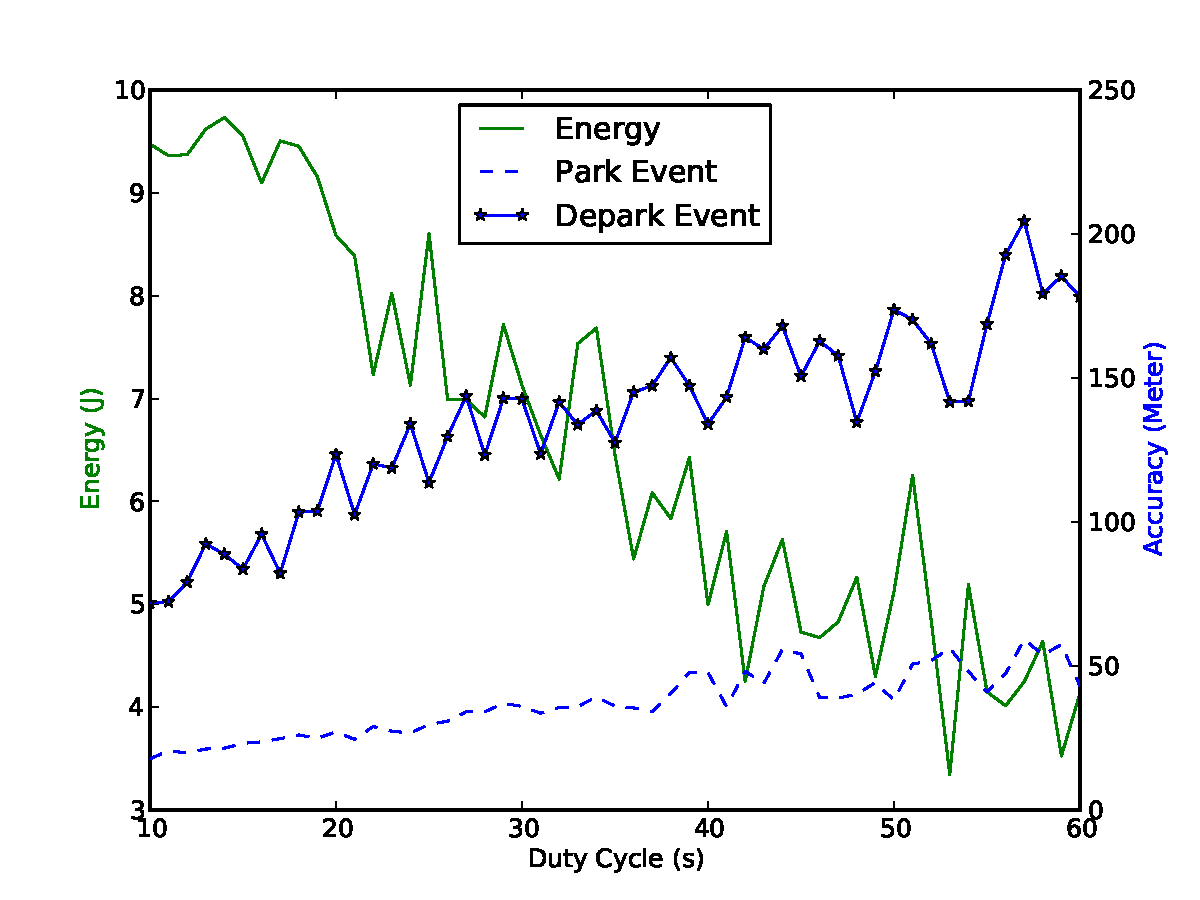
\includegraphics[width=3.325in]{./figures/Energy_accuracy.pdf}

\caption{\textbf{Power usage vs. detector accuracy.} Energy usage by
PocketParker is low at all duty cycles, so we chose a high duty cycle in
order to improve detection accuracy.}

\label{fig-energy}
\end{figure}

\newcolumntype{b}{>{\hsize=1.4\hsize}X}
\newcolumntype{s}{>{\hsize=.6\hsize}X}
\begin{table}[t]
{\small
\begin{threeparttable}
\begin{tabularx}{\columnwidth}{b s b s}
  {{\textbf{Carry Location}}} & {{\textbf{Count}}} &
  {{\textbf{Car Location}}} &
  {{\textbf{Count}}} \\
 \hline
In hand & 18 & Cup holder & 16 \\
Side bag & 10 & Car seat  & 9 \\
Back pack & 10 & Side bag & 10 \\
In hand talking & 7 & Back pack & 9 \\
Front pocket & 14 & Front pocket & 14 \\
Jacket pocket & 14 & Jacket pocket & 14 \\
Back pocket & 7 & Back pocket & 14 \\
\end{tabularx}
\end{threeparttable}
\caption{\textbf{Carry and car location for detector experiment.}
Eight participants generated 80 runs, carrying and placing the
phone in their car in many ways.}
\label{table-experiment}
}
\vspace*{-0.1in}
\end{table}


To determine the right parameter settings for our transition detector, we
conducted a controlled experiment. During this experiment, accelerometer and
GPS data was collected and stored continuously on each device, and
participants were asked to manually label each transition into and out of the
car. Afterwards, data was processed by a Python simulator implementing the
identical algorithm used by the PocketParker application, allowing us measure
accuracy and energy consumption as a function of the detector duty cycle.

Eight volunteers participated, including seven men and one woman. Seven were
right-handed and one was left-handed. Each was asked to conduct the same
experiment ten times: (1) carrying the instrumented phone, walk to their car;
(2) label departure; (3) drive around campus briefly; (4) park and label
arrival; (5) return inside. Since the way the phone is carried while walking
and placed in the car while driving affects the accelerometer readings, care
was taken to generate a good mix of carry and car location styles.
Table~\ref{table-experiment} shows the breakdown. The experiment permitted us
to obtain sensing data from a cross section of individuals possessing
different body morphologies, habits of driving cars, and ways of handling
mobile devices. Participation in the experiment took roughly one hour and
pizza was provided.

Figure~\ref{fig-energy} displays the tradeoff between energy usage and
detection accuracy as a function of the PocketParker duty cycle. Here we
combine an active period of 5s with a inactive period of variable length,
between 5~and~55s, for an overall duty cycle between 0.5 and 0.06. Our
simulator uses energy numbers used by the Android Fuel Guage application
along with the acceloremeter duty cycles and number of GPS locations
requested including false positives to estimate average power consumption.
This graph measures the accuracy of detected events in terms of distance from
the actual location of the event labeled by the participant.

As we expect, longer duty cycles consume less energy but produce longer
detection latencies which translate into higher distances from the event
location. Note also that the departure events have higher location error than
the parking events, because departing users are driving and therefore
traveling more rapidly. Overall power usage by PocketParker is low, under
10~mW at all duty cycles. Because PocketParker's ability to map parking
events into lots is affected by the detection distance accuracy, we chose a
low total period of 15~s for a 0.25 duty cycle. This allows PocketParker to
determine location to within 25~m for parking events and 80~m for departures.
Power consumption at this duty cycle is 8~mW, representing 4.2\% of the
capacity of a 1500~mAh battery over 24~hours of usage.

\begin{figure}
\centering
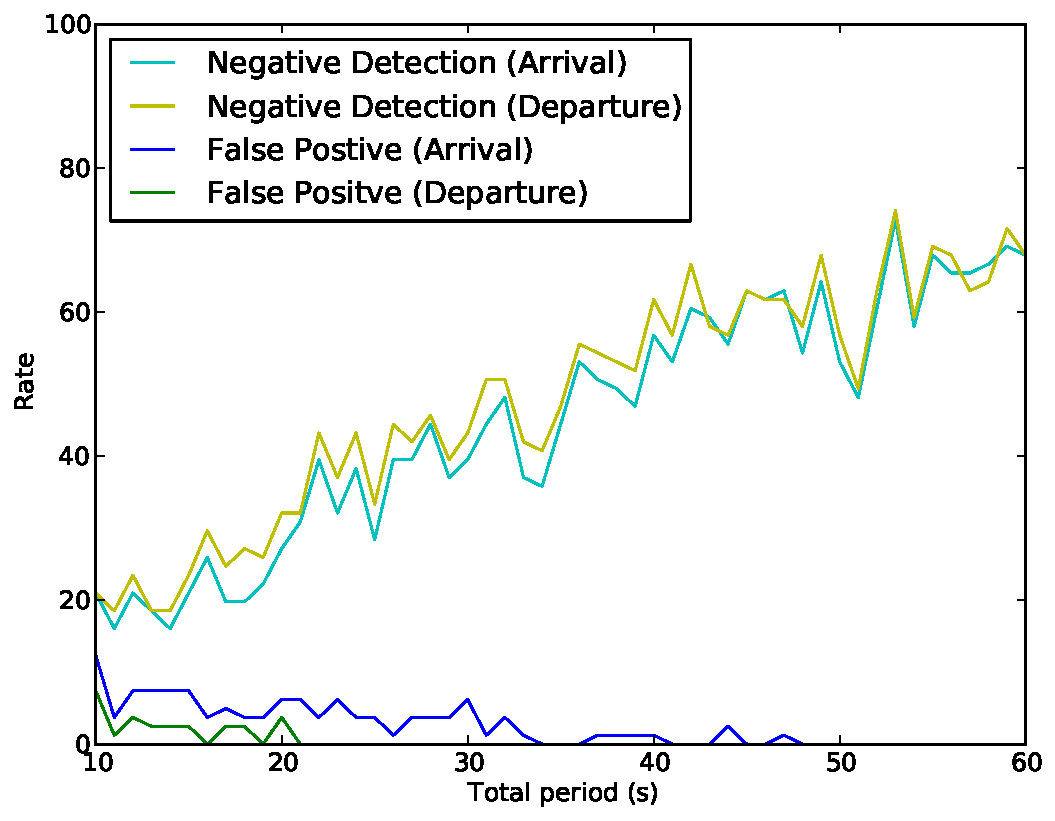
\includegraphics[width=3.325in]{./figures/Rate_FP_and_ND.pdf}

\caption{\textbf{False positive and negative rates as a function of detector
duty cycle.}} 

\label{fig-falsepositives}
\end{figure}

Using the same data we also examine the false positive and negative rates for
arrivals and departures. This is important since, without explicit user
input, it would be impossible to determine this information while
PocketParker is in use. Figure~\ref{fig-falsepositives} shows PocketParker
can detect 80\% of arrival and departure events correctly at the 0.25 duty
cycle we use. False positive rates are already quite low, and this is before
we apply our GPS availability filter and lot location filters. False
positives decline as the duty cycle decreases because PocketParker has fewer
opportunities to detect user activity.

\subsection{Simulation Results}
\label{subsec-simulator}

To experiment with PocketParker in a more controlled setting, we implemented
a parking lot simulator in Python. Our simulator allows us to simulate any
number of parking lots associated with any number of points of interest with
varying desirability levels. For simplicity during our evaluation, we
simulate two lots 1~and~2 with lot~1 filling before lot~2, although lot
choice by simulated drivers is randomly weighted. Particularly for evaluating
our monitored fraction estimation, we use five types of lots that fill and
empty differently:

\begin{itemize}

\item \textbf{Fast Fill} and \textbf{Slow Fill} fill once per day quickly or
slowly, like a lot associated with a place of work.

\item \textbf{High Churn} starts with lot~1 full and experiences continuously
high arrival and departures rates, like an airport parking lot.

\item \textbf{Low Churn} represents underutilized lots that never completely
fill, with lot~2 almost completely unused.

\item \textbf{Multiple Fill} represents a lot that rapidly fills and empties
repeatedly during each day, like a campus lot or movie theater.

\end{itemize}

Figure~\ref{fig-lotsdescription} shows the arrival and departure rates for
each of the types of lot as well as the resulting per-lot capacity.

\begin{figure*}
\centering
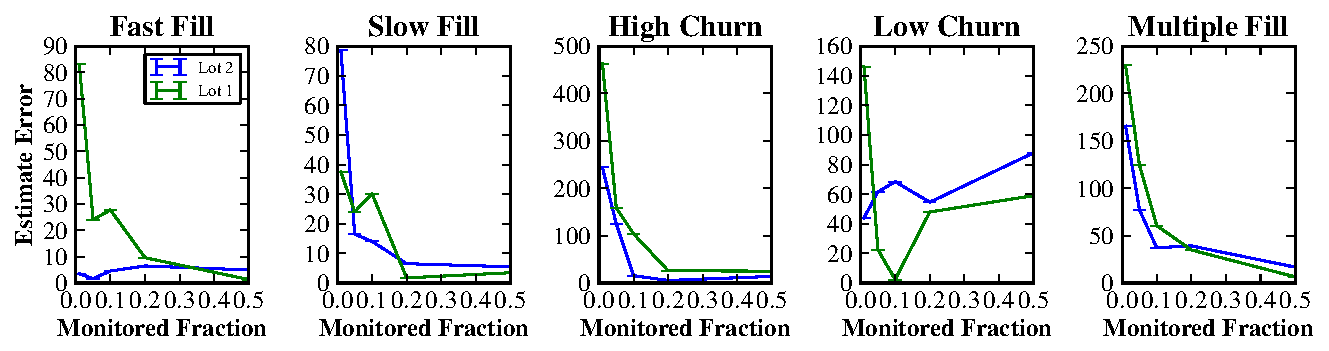
\includegraphics[width=\textwidth]{./simulator/figures/capacity_experiment.pdf}

\caption{\textbf{Errors in monitored fraction estimation.} Currently
PocketParker is better at estimating the monitored fraction when lots fill
and empty regularly.}

\label{fig-capacityerrors}
\end{figure*}

\subsubsection{Monitored fraction estimation}

In Section~\ref{subsubsec-monitored} we describe our approach to estimated
the monitored fraction, a parameter important to the operation of the
PocketParker availability estimator. Figure~\ref{fig-capacityerrors} shows
the results of 10 random simulations for each lot type. In each case, the
monitored fraction estimator uses a weeks worth of data and proceeds as
described previously. The error in the monitored fraction estimate is shown
as a function of the actual monitored fraction for the simulation used.

For the five types of lots, we would expect PocketParker to do better
monitored fraction estimation when lots fill regularly---Fast Fill, Slow
Fill, and Multiple Fill---and poorly when they do fill erratically or not at
all---High and Low Churn. The results in Figure~\ref{fig-capacityerrors}
generally follow this pattern. Errors for High Churn are quite high, and Low
Churn errors persist even at high monitored driver fractions. This is
natural, as the Low Churn lot never fills. Fast Fill results improve with
increasing monitored driver fraction. We are investigating, however, the
problems with estimating lot~1 capacity, and persistent errors with the Slow
Fill lots. Improving the accuracy of monitored fraction estimation may
require additional smoothing techniques or merging information from multiple
related lots. However, as we demonstrate later, our availability estimator is
robust to monitored fraction estimation errors up to 50\%.

\begin{figure}[t]
\centering
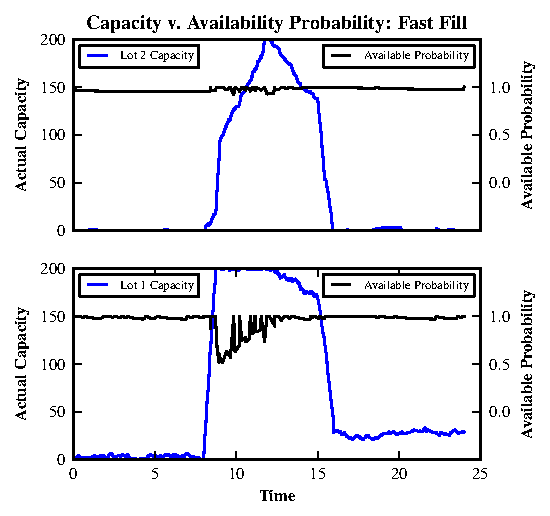
\includegraphics[width=3.325in]{./simulator/figures/tracking_fastfill.pdf}

\caption{\textbf{Availability probabilities tracking lot capacity.} Dips in
the availability probability correspond to times when PocketParker believes
the lot is full. Discontinuities are caused by departures, which set the
instantaneous probability that the lot is available to 1.0.}

\label{fig-trackingexample}
\end{figure}

\subsubsection{Probability and availability}

At this point we take a closer look at the way that PocketParker adjusts lot
availability probabilities. Keep in mind that the absolute value of the
availability probability for each lot may not meaningful. Instead,
PocketParker uses the probabilites to order available lots in response to
queries. We examine its accuracy at performing this essential task next.
However, it is illustrative to examine the probabilities PocketParker
maintains and observe how they vary as the number of available spots in the
lot changes.

Figure~\ref{fig-trackingexample} shows a 24~hour simulation of a Fast Fill
parking lot with a monitored fraction of 0.1 and a 10\% error in the
estimation of the monitored fraction. The ground truth capacity of the lot as
simulated is plotted next to the PocketParker probability that the lot has an
available spot. At the beginning of the simulation, both lots are marked as
free. When lot~1 fills and lot~2 begins to fill, generating implicit searches
in lot~1, the availability probability of lot~1 drops. It spikes upward
repeatedly due to departures from lot~1---which reset the short-term
probability of an available spot back to 1---but does not equal the
probability for lot~2 again until the point when the departure rate for lot~1
climbs.

\subsubsection{Prediction accuracy}

\begin{table}[t]
\begin{threeparttable}
{\small
\begin{tabularx}{\columnwidth}{Xrrrrr}
\multicolumn{1}{c}{\textbf{Type}} & 
\multicolumn{1}{c}{\textbf{$f_m$}} & 
\multicolumn{1}{c}{\textbf{$f_m$ Error}} & 
\multicolumn{1}{c}{\textbf{Correct}} & 
\multicolumn{1}{c}{\textbf{Missed}} & 
\multicolumn{1}{c}{\textbf{Waste}}\\ \toprule

\textbf{Campus} & & & & & \\
\midrule
& 0.20 & 0.10 & 100.0 \% & 0.0 \% & 0.0 \% \\
\textbf{Fast Fill} & & & & & \\
\midrule
& 0.01 & 0.10 & 75.1 \% & 24.7 \% & 0.2 \% \\
& 0.05 & 0.10 & 72.3 \% & 26.2 \% & 1.5 \% \\
& 0.10 & 0.10 & 80.0 \% & 15.6 \% & 4.4 \% \\
& 0.10 & 0.20 & 86.6 \% & 11.2 \% & 2.2 \% \\
& 0.10 & 0.50 & 89.7 \% & 7.7 \% & 2.7 \% \\
& 0.10 & 1.00 & 93.0 \% & 4.8 \% & 2.2 \% \\
& 0.20 & 0.10 & 87.9 \% & 8.5 \% & 3.6 \% \\
& 0.50 & 0.10 & 94.0 \% & 5.0 \% & 1.0 \% \\
\textbf{High Churn} & & & & & \\
\midrule
& 0.01 & 0.10 & 54.0 \% & 0.0 \% & 46.0 \% \\
& 0.05 & 0.10 & 55.3 \% & 0.0 \% & 44.7 \% \\
& 0.10 & 0.10 & 63.6 \% & 0.0 \% & 36.4 \% \\
& 0.10 & 0.20 & 62.2 \% & 0.0 \% & 37.8 \% \\
& 0.10 & 0.50 & 60.1 \% & 0.0 \% & 39.9 \% \\
& 0.10 & 1.00 & 61.8 \% & 0.0 \% & 38.2 \% \\
& 0.20 & 0.10 & 64.0 \% & 0.0 \% & 36.0 \% \\
& 0.50 & 0.10 & 70.6 \% & 0.0 \% & 29.4 \% \\
\textbf{Low Churn} & & & & & \\
\midrule
& 0.01 & 0.10 & 98.4 \% & 0.0 \% & 1.6 \% \\
& 0.05 & 0.10 & 89.1 \% & 0.0 \% & 10.9 \% \\
& 0.10 & 0.10 & 94.1 \% & 0.0 \% & 5.9 \% \\
& 0.10 & 0.20 & 91.0 \% & 0.0 \% & 9.0 \% \\
& 0.10 & 0.50 & 87.9 \% & 0.0 \% & 12.1 \% \\
& 0.10 & 1.00 & 87.8 \% & 0.0 \% & 12.2 \% \\
& 0.20 & 0.10 & 92.5 \% & 0.0 \% & 7.5 \% \\
& 0.50 & 0.10 & 91.6 \% & 0.0 \% & 8.4 \% \\
\textbf{Multiple Fill} & & & & & \\
\midrule
& 0.01 & 0.10 & 51.4 \% & 42.8 \% & 5.8 \% \\
& 0.05 & 0.10 & 71.2 \% & 26.0 \% & 2.9 \% \\
& 0.10 & 0.10 & 85.2 \% & 13.2 \% & 1.6 \% \\
& 0.10 & 0.20 & 79.4 \% & 17.5 \% & 3.1 \% \\
& 0.10 & 0.50 & 86.2 \% & 12.7 \% & 1.1 \% \\
& 0.10 & 1.00 & 77.6 \% & 20.9 \% & 1.5 \% \\
& 0.20 & 0.10 & 92.1 \% & 7.5 \% & 0.5 \% \\
& 0.50 & 0.10 & 91.6 \% & 7.8 \% & 0.6 \% \\
\textbf{Slow Fill} & & & & & \\
\midrule
& 0.01 & 0.10 & 70.7 \% & 26.0 \% & 3.2 \% \\
& 0.05 & 0.10 & 78.8 \% & 17.5 \% & 3.7 \% \\
& 0.10 & 0.10 & 82.1 \% & 13.3 \% & 4.6 \% \\
& 0.10 & 0.20 & 75.4 \% & 15.2 \% & 9.4 \% \\
& 0.10 & 0.50 & 80.5 \% & 19.3 \% & 0.2 \% \\
& 0.10 & 1.00 & 85.2 \% & 12.5 \% & 2.3 \% \\
& 0.20 & 0.10 & 87.8 \% & 9.8 \% & 2.4 \% \\
& 0.50 & 0.10 & 93.8 \% & 5.6 \% & 0.6 \% \\
\end{tabularx}
}
\caption{\textbf{Accuracy of PocketParker predictions for various kinds of lots and parameters.}}
\label{table-accuracy}
\end{threeparttable}
\end{table}


PocketParker exists to help drivers choose parking lots. Here, we examine our
simulation results and determine whether we accomplish this goal. In our
simulations, we inject regular queries to PocketParker asking it to order the
two available lots. We categorize its response as either a correct
prediction, a missed opportunity, or a waste of time. A missed opportunity
represents a case where a more desirable lot was available than the one that
PocketParker recommended. A waste of time indicates that PocketParker sent
the user to a lot that did not actually have an available spot.

Table~\ref{table-accuracy} shows data from simulations run on several
different lot types and while varying simulation parameters including the
monitored fraction $f_m$ and estimation error in the monitored fraction. At
regular timesteps we query PocketParker and ask it to order the two lots
lot~1 and lot~2. We then compare its ordering with the ground truth available
through the simulator. In the case that two lots have probabilities within
$0.01$ of each other, PocketParker considers this a tie and suggests the more
preferable lot first.

Several trends can be observed in the results. First, overall PocketParker
does well on most lot types. The High Churn lot presents the greatest
difficulty, which we would expect since its large number of incoming and
outgoing drivers make prediction difficult. We are also concerned that the
High Churn errors are exclusively waste, indicating that PocketParker is
consistently sending drivers to the wrong lot, probably because it is
predicting that spots are available longer than they actually are. Clearly
more work is needed to determine the right approach for High Churn lots.

Excluding the High Churn lot, the lowest correct percentage with a $f_m >
0.1$ is 75\% for the Slow Fill lot, and accuracy is good throughout. The Low
Churn lot has a small number of errors but this is because both lots are
usually empty. Its error breakdown is similar to the High Churn lot, which
suggests it is something about regular departures and arrivals that is
causing PocketParker to be too optimistic about availability in the more
desirable lot.

Note, however, that this uniform query pattern is the most challenging for
PocketParker and so these results may be seen as a lower bound. This is
because PocketParker has the most information about lot availability during
active periods of arrival and departure events. Once it stops receiving
information, uncertainty grows. So to the degree that PocketParker queries
follow at least to some degree the pattern of arrivals and departures, we
will have fresh data and do well.

\subsection{Deployment}

\begin{figure*}
\centering
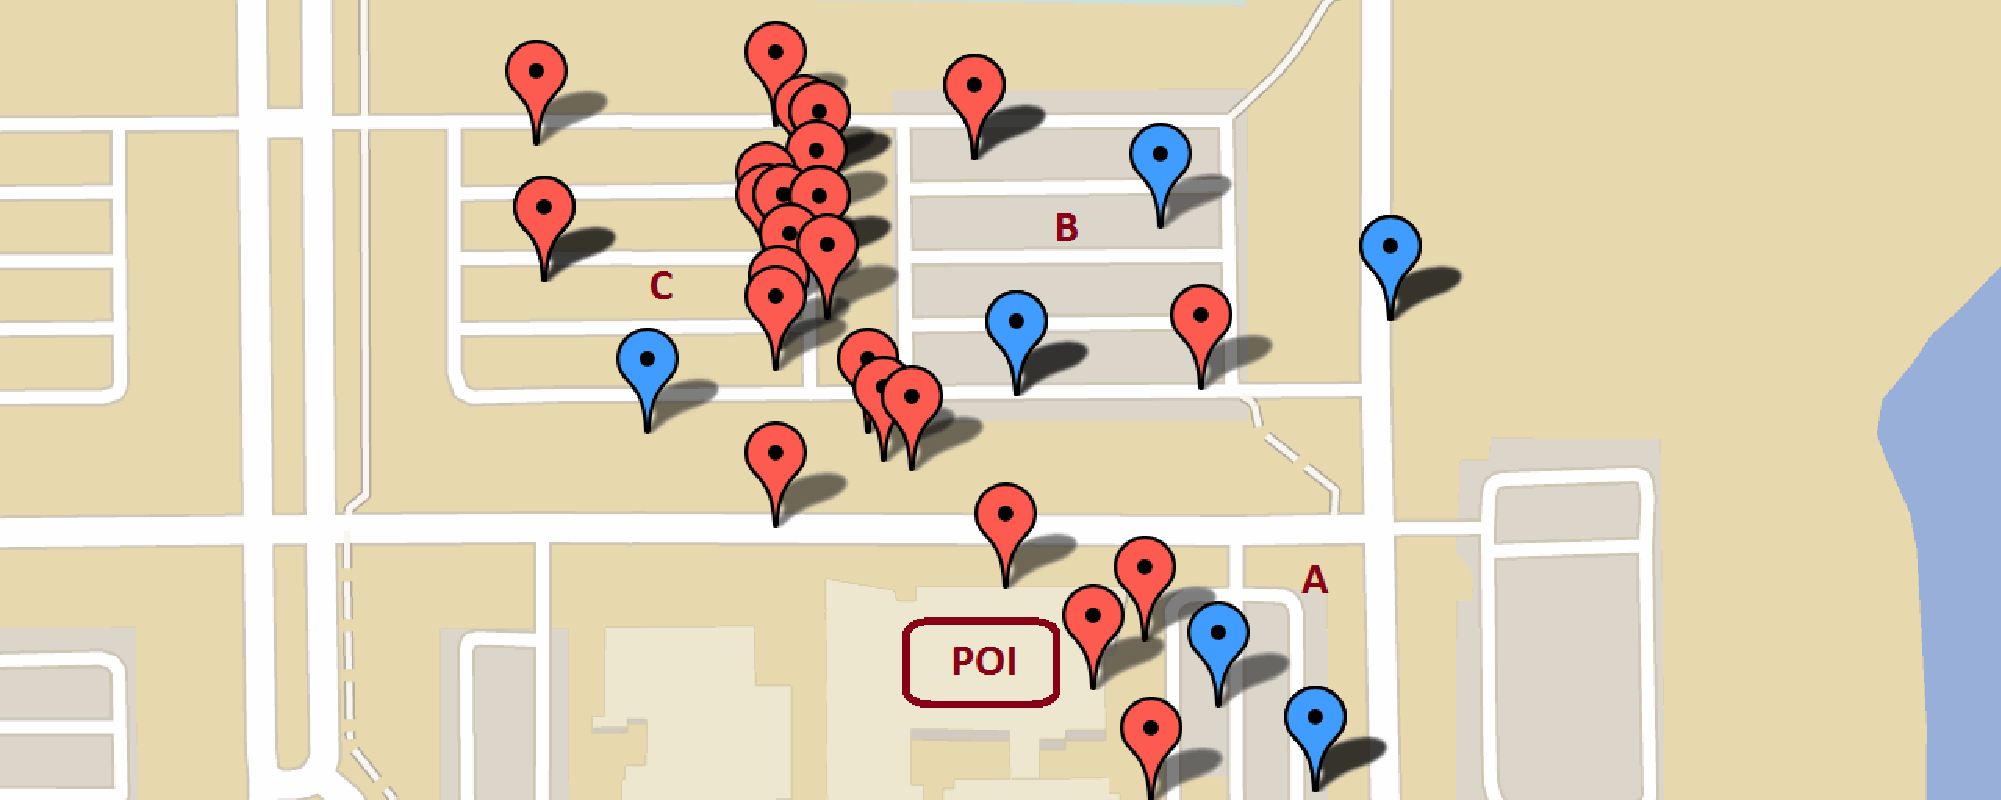
\includegraphics[width=\textwidth]{./figures/detectedEventsOnMap.pdf}

\caption{\textbf{Map showing all events detected by PocketParker during our
ten-day deployment.} 56~events are shown in three monitored lots. Red markers
indicate arrivals, blue departures. Lots~A~and~B were monitored by cameras to
establish ground truth, and Lot~A is considered the most desirable of the
three lots.}

\label{fig-events}
\end{figure*}

Finally, to establish the accuracy of PocketParker we performed a small-scale
deployment on our university campus. We implemented a PocketParker client as
an Android application for Android version 4.1 ``JellyBean''. We tested our
app on Samsung Nexus~S~4G smartphones, but PocketParker should be able to run
on any smartphone with GPS and an accelerometer, and on previous versions of
Android. Other than the PocketParker server which receives events and updates
the availability estimate, no infrastructure is required.

We recruited five participants that installed our PocketParker application
and generated 372 events over ten days---202 arrivals and 170 departures. Of
those events, 127 occurred near campus including false positives, and 56 were
mapped into the three campus lots monitored by PocketParker\footnote{One
participant lives quite close to campus, and many of the parking transitions
that occurred at their house were included in the 71~events near campus that
did not map into known parking lots.}. The deployment period included several
days when participants did not come to campus, and most parking events were
generated by three participants who came to campus daily. No participants
complained of excessive energy usage or battery life degradation, and no
interaction with the application was required.

Figure~\ref{fig-events} shows all of the events that occurred in the three
lots we monitored. Our computer science department is labeled as the point of
interest. To determine the ground truth availability of the monitored lots we
positioned four cameras at locations within the building to monitor lots
A~and~B in Figure~\ref{fig-events}. Despite the fact that many parking events
took place in lot~C, we were unable to locate a suitable unobstructed vantage
point to gather camera data. We used Nexus~S~4G smartphones equipped with
fish-eye lenses as cameras. Each took time lapse images at 1~Hz, time-stamped
them using NTP and uploaded them to a central server. Figure~\ref{fig-camera}
shows two of our cameras and a view of one of the monitored parking lots. A
total of 36,000 images were collected for all four parking lots over two
weeks.

To measure capacity, one day's worth of images for two lots was hand-coded on
a ten-point scale at ten-minute intervals. Because we are particularly
interested in the transition between empty and full states, we were careful
to ensure that the lot was never marked completely full if there was a single
available spot visible. Because we collected a relatively-small number of
parking events into camera-monitored lots A~and~B during our deployment, we
merge all events into a single day before feeding the events into the
PocketParker estimation engine. Given the location of other campus buildings
to the south of our building, lot~A is considered more desirable than lot~B.

Table~\ref{table-accuracy} also includes numbers for our campus deployment
labeled as ``Campus''. Because we do not know the monitored fraction, we
experiment with several different values. Overall the accuracy of
PocketParker is excellent, even achieving 100\% accuracy at a monitored
driver fraction of 0.2. We believe this is because the more preferable
monitored lot has a very predictable availability pattern, filling rapidly
and staying full during business hours.

\begin{figure}[t]
\centering
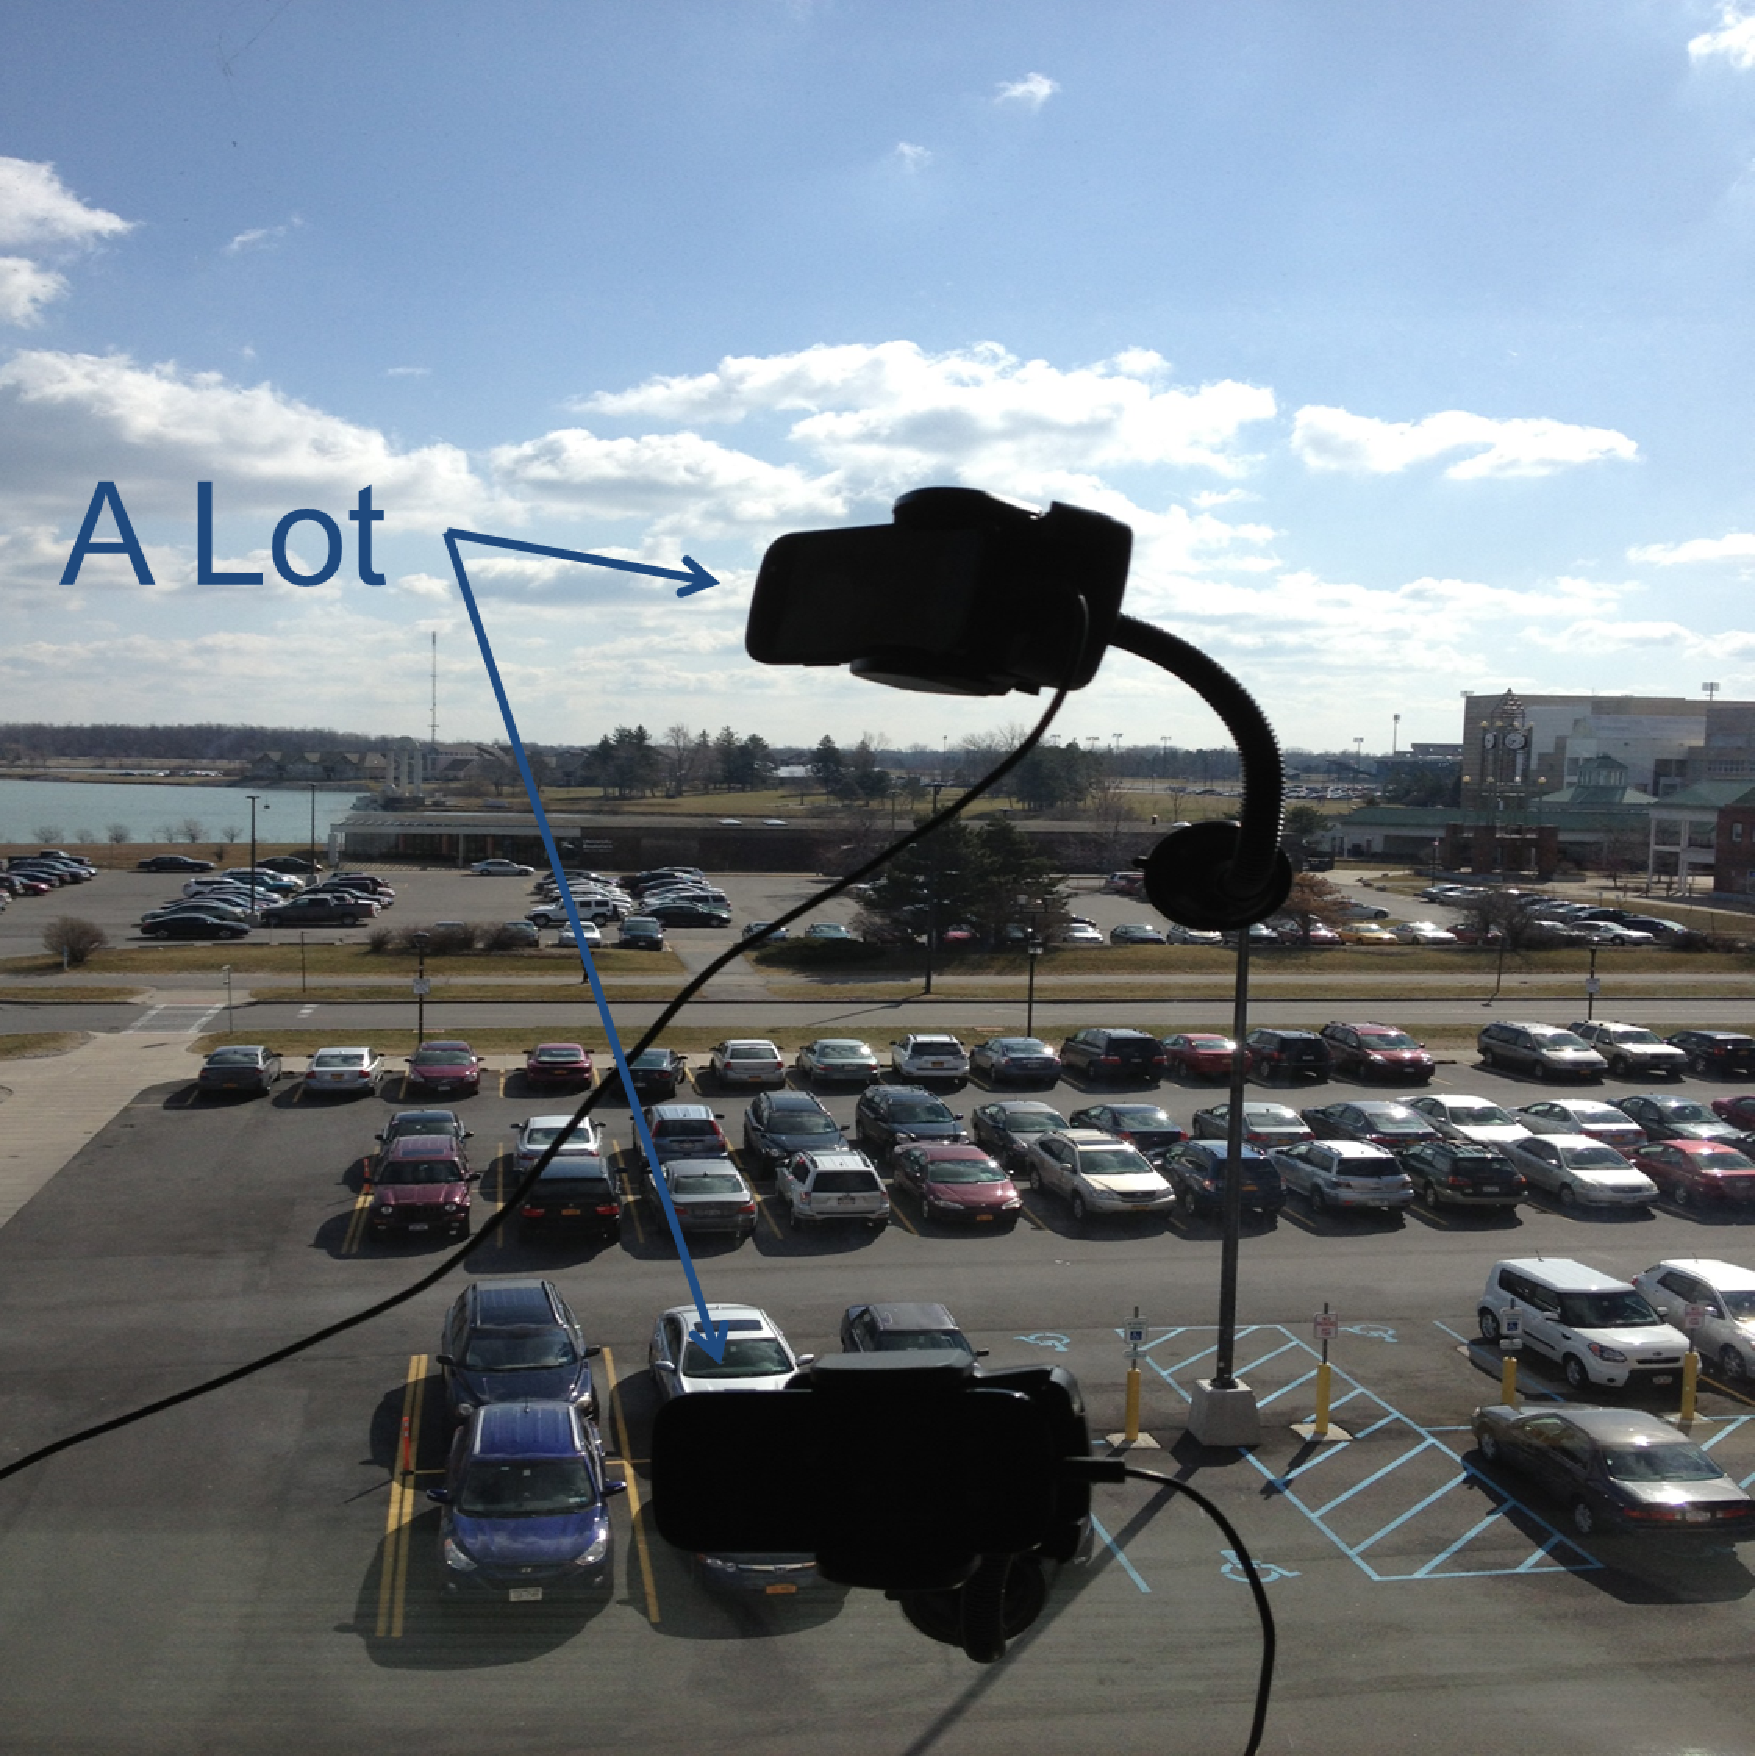
\includegraphics[width=3.0in]{./figures/Camera_setting.pdf}

\caption{\textbf{Monitoring cameras.} A view of one of the monitored parking
lots is shown.}

\label{fig-camera}
\end{figure}
